\chapter{Fonctionnement générale du système }
\phantomsection
\addcontentsline{toc}{chapter}{Fonctionnement générale du système} 

\section{Introduction}

Dans ce chapitre, nous allons présenter en détail la conception et la réalisation de notre système de suivi en temps réel des batteries solaires. Nous expliquons les choix technologiques et les méthodes employées pour mesurer et surveiller les paramètres critiques abordés dans le chapitre précédent.

\subsection{Présentation générale du dispositif} Le dispositif est conçu pour surveiller en temps réel les paramètres essentiels de trois batteries solaires utilisées dans une installation photovoltaïque. Ce système capture des données telles que la tension, le courant et la température de chaque batterie individuellement, que les batteries soient montées en série ou en parallèle. Il fournit également des informations sur l'état de charge (SoC) et l'état de décharge (DoD) du système. En cas d'anomalie, le dispositif peut envoyer une alerte par SMS ou par email via l'application web, grâce à l'utilisation d'un microcontrôleur.

\subsection{Analyse des besoins du dispositif} 
Avant de concevoir le dispositif, il est essentiel de comprendre ses besoins spécifiques. Voici les exigences pour notre dispositif :

\begin{itemize} 
	\item Informations sur les paramètres de chaque batterie : 
	\begin{itemize} 
		\item Tension 
		\item Courant 
		\item Température 
	\end{itemize}
	\item Traitement des informations de chaque batterie et de l'ensemble du système 
	\item Envoi des données vers un système de stockage en ligne 
	\item Visualisation des données stockage 
	\item Alertes en cas de dysfonctionnement de la batterie 

\end{itemize}


\subsection{Architecture générale du système}

Pour bien visualise notre système en générale on peut classer les besoins par plusieurs bloc fonctionnels. 

%Les capteurs collectent les informations des trois batteries solaires, telles que la tension, le courant et la température. Ces données sont ensuite transmises au bloc de traitement, où elles sont analysées et prétraitées. Les données traitées sont envoyées à un serveur de stockage en ligne pour être enregistrées. Les informations stockées sont utilisées par l'application de surveillance, qui permet de visualiser les paramètres des batteries et de gérer les alertes. La figure suivante illustre l'architecture générale du système.


\begin{figure}[H]
	\centering
	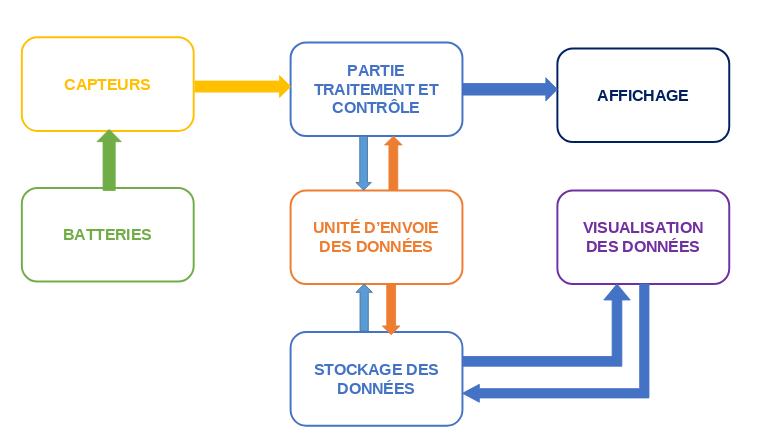
\includegraphics[width=17cm]{./img/schemaBloc.png}
	\caption{Schéma bloc du système générale }
	\label{i1}
	
\end{figure}

Le système est compose par sept bloc distinct avec leurs fonctionnement précise. Alors on va voire l'explication chaque bloc :

\paragraph{Bloc batterie : }
 celui ci est constituer par 3 batteries que le dispositif doit surveiller en temps réel.
 
\paragraph{Bloc des capteurs : }
 
Ce le bloc qui fournit les informations vers l'ensemble du systeme . Il est constitue par  des capteurs suivants :
\begin{itemize}
	\item Capteur de tension : Mesure la tension de chaque batterie.
	\item Capteur de courant : Mesure le courant de charge et de décharge de chaque batterie.
	\item	Capteur de température : Mesure la température de chaque batterie.
\end{itemize}

\paragraph{Unité de traitement et contrôle : }


Ce bloc est le cerveau de notre dispositif car il traite les informations reçues du bloc précèdent , effectuant les calculs nécessaire et convertir les données analogiques en valeurs compréhensibles par les machines, et stock les programmes nécessaires au fonctionnement du système.

\paragraph{Bloc d'affichage :}
Il est destiné a afficher les informations que le bloc precedent décide d'afficher. 

\paragraph{Unité d'envoie de données : }
il jout le role de transmission de données que le bloc de traitement a été traité et qu'il décide d'envoyer .

\paragraph{Centre de stockage  :}
Ce partie stocke les informations pré-traitées pour qu'elles puissent être utilisées pour surveiller l'état des batteries. Le stockage permet également de conserver un historique des données pour des analyses ultérieures.

\paragraph{Bloc de visualisation de données:}
C'est pour visualiser les données en temps réel que le bloc de stockage stock .

C'est une plateforme en ligne qui permet de visualiser en temps réel les tensions, courants, températures de chaque batterie ainsi que de l'ensemble du système. Cette plateforme offre également d'autres fonctionnalités comme la gestion des alertes et l'analyse des données historiques.
Pour bien comprendre l'architecture du système, la figure suivante présente une vue détaillée des composants et de leur interaction.

\begin{figure}[H]
	\centering
	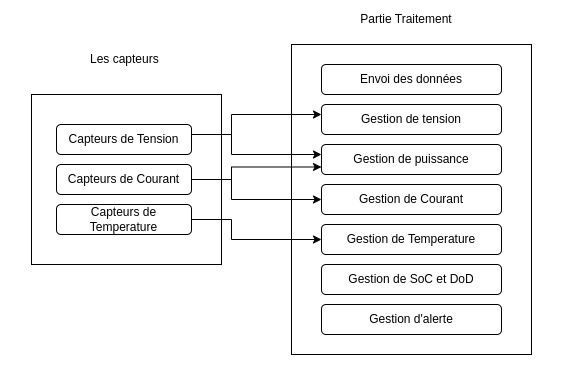
\includegraphics[width=15cm]{./img/schemaFonctionnel.png}
	\caption{Bloc de fonctionnement du système }
	\label{i1}
	
\end{figure}

\subsection*{Système de gestion de la température}
La température a une influence majeure sur le comportement de la batterie en termes de charge et de décharge. Lorsque la température baisse, la capacité de la batterie diminue également. En revanche, lorsque la température revient à la normale, la capacité retrouve son niveau habituel. À l'inverse, une augmentation de la température entraîne une augmentation de la capacité de la batterie.\\

\noindent Toutes ces variations de température affectent la durée de vie de la batterie. C'est pourquoi il est essentiel de surveiller la température de la batterie pour remédier à ces problèmes.
\\

\begin{figure}[H]
	\centering
	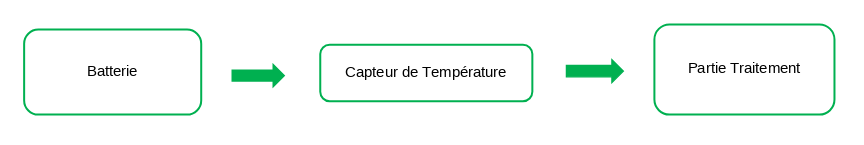
\includegraphics[width=17cm]{./img/capteurTemperature.png}
	\caption{Système de contrôle de température }
	\label{i1}
\end{figure}

Le capteur collecte les données de la batterie et vérifie d'abord si la température ne dépasse pas les seuils critiques Tcmin et Tcmax. Si ces seuils sont franchis, une alerte est envoyée à l'utilisateur.
La figure ci-dessous présente un logigramme explicatif du système.

\begin{figure}[H]
	\centering
	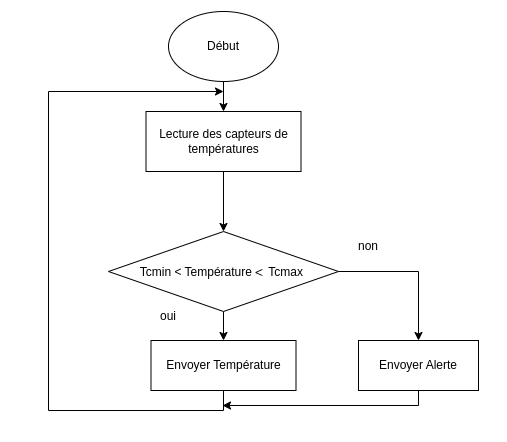
\includegraphics[width=12cm]{./img/LogigrammeDuSystemeTemperature.png}
	\caption{Logigramme du système de contrôle de température }
	\label{i1}
\end{figure}

\subsection*{Le capteur de température DS18B20} 
Le capteur thermique numérique DS18B20 est assez précise et ne nécessite aucun composant externe pour fonctionner. Il peut mesurer les températures de -55 ° C à + 125 ° C avec une précision de mesure de ± 0,5 ° C.
La résolution du capteur de mesure est configurable par l'utilisateur sur 9, 10, 11 ou 12 bits. Cependant, la résolution par défaut à la mise sous tension est de 12 bits (soit une précision de 0,0625 ° C).
\\

\noindent Cet instrument de mesure peut être alimenté avec une alimentation de 3 V à 5,5 V et ne consomme que 1 mA lors des conversions de températures actives.
\\

\noindent Voici les spécifications complètes du capteur de température numérique DS18B20: 

\begin{filleditem}
	\item Source de courant	: 3 V à 5,5 V
	\item Consommation de courant :	1mA
	\item Page de température :	-55 à 125 ° C
	\item Précision : 	± 0,5 ° C
	\item Résolution :	9 à 12 bits (sélectionnable)
	\item Temps de réponse :	<750 ms
\end{filleditem}
\begin{figure}[H]
	\centering
	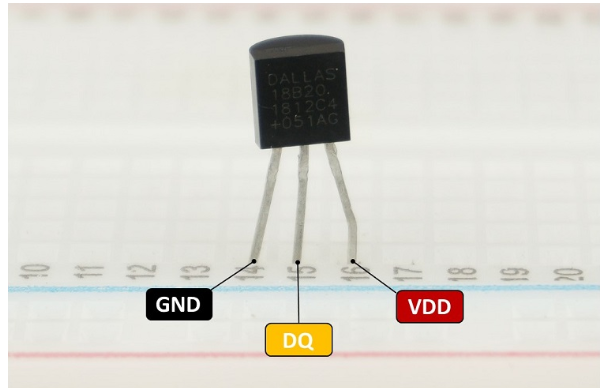
\includegraphics[width=6cm]{./img/DS18B20.png}
	\caption{Capteur de température DS18B20 }
	\label{i1}
\end{figure}

\begin{table}[H]
	\centering
	\caption{Explication des broches du DS12B20  } \vspace{5mm}
	\begin{tabular}[c]{|p{4cm}|p{10cm}|}
				
		\hline
		\rule[0.5cm]{0cm}{0cm} Noir	& GND est une broche de terre
		\\
		\hline
		\rule[0.5cm]{0cm}{0cm} Jaune &	Le DQ est un bus de données à 1 fil qui doit être connecté à une broche numérique sur le microcontrôleur.

		\\
		\hline
		\rule[0.5cm]{0cm}{0cm} Rouge &	La broche VDD fournit une alimentation au capteur qui peut être comprise entre 3,3 et 5 V.
		\\
		\hline
	
		
	\end{tabular}
\end{table}	


\subsection*{Avantage}
L'un des plus grands avantages du DS18B20 est que plusieurs DS18B20 peuvent coexister sur le même bus 1 fil. Cela signifie qu'il n'a besoin que d'une seule ligne de données (et de GND) pour communiquer avec le microcontrôleur .\\
Comme chaque DS18B20 possède un code série 64 bits unique gravé en usine, il est plus facile de les différencier les uns des autres.Cette fonctionnalité peut être un énorme avantage pour contrôler de nombreux DS18B20 répartis sur une grande surface. 
\\

Il y a deux mode que celui ci peut tirer son énergie :
\begin{itemize}
	\item une source d'alimentation externe (appelé «\textbf{ mode normale} »)
	\item la ligne de données elle-même (appelé «\textbf{ mode parasite} »), éliminant ainsi le besoin d'une alimentation externe.
\end{itemize}

\begin{figure}[H]
	\centering
	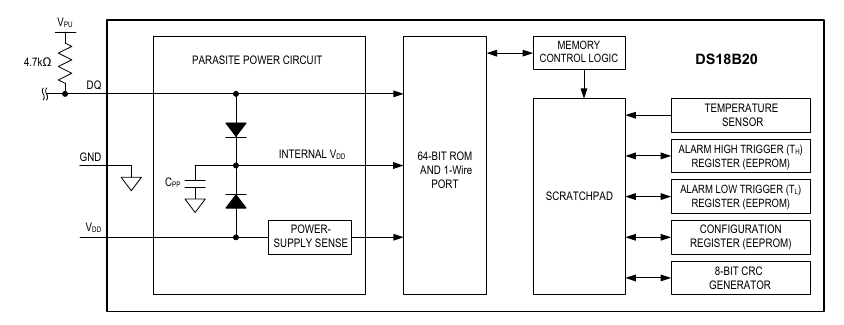
\includegraphics[width=15cm]{./img/blocDiagramDS18B20.png}
	\caption{Diagramme bloc du Capteur de température DS18B20 }
	\label{i1}
\end{figure}

\subsection*{Système de gestion de la tension et du courant}
Les batteries solaires fournissent une tension et une intensité dans une plage prédéfinie. Il est essentiel de surveiller ces paramètres en temps réel pour protéger les batteries et assurer leur bon fonctionnement. La surveillance de la tension et du courant permet également de calculer la puissance de la batterie ainsi que l'état de charge (SoC) et l'état de décharge (DoD).
\\

\begin{filleditem}
	\item \textbf{Tension} : La tension est un indicateur clé de l'état de la batterie. Une tension trop basse peut indiquer une décharge excessive, tandis qu'une tension trop élevée peut signaler une surcharge, ce qui peut endommager la batterie.
	\item	\textbf{Courant} : L'intensité du courant permet de déterminer le flux d'énergie entrant et sortant de la batterie. Des courants trop élevés peuvent surcharger la batterie, tandis que des courants trop faibles peuvent indiquer un problème de connexion ou un dysfonctionnement.
	\item	\textbf{Puissance} : La puissance fournie par la batterie est calculée à partir de la tension et du courant (P = V * I). La connaissance de la puissance permet de déterminer la capacité de la batterie à fournir de l'énergie aux charges connectées et d'optimiser l'utilisation des ressources énergétiques.
\end{filleditem}	
\subsection*{Architecture du système de gestion de la tension et du courant}
Les capteurs de tension et de courant mesurent en temps réel la tension et l'intensité de chaque batterie. Les données sont ensuite transmises au centre de traitement pour une analyse continue.

\begin{figure}[H]
	\centering
	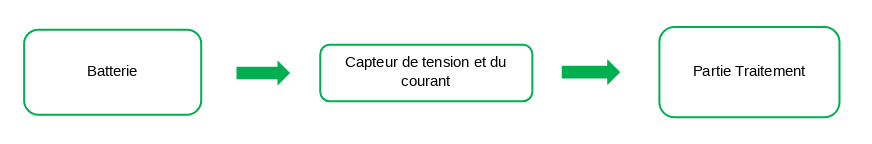
\includegraphics[width=17cm]{./img/capteurTensionCOurant.png}
	\caption{Système de contrôle de la tension et du courant }
	\label{i1}
\end{figure}

\subsection*{Module de capteur de courant continu INA226}
L'INA226 est un moniteur de courant et de tension doté d'une interface compatible I2C ou SMBUS. Il permet de surveiller à la fois la chute de tension à travers un shunt et la tension du bus d'alimentation. Grâce à une valeur d'étalonnage programmable, des temps de conversion configurables et un calcul de la moyenne, l'INA226 permet des lectures directes du courant en ampères et de la puissance en watts \cite{6}.\\

Cet appareil peut détecter le courant sur des tensions de bus allant de 0V à 36V, indépendamment de la tension d'alimentation. Il fonctionne à partir d'une seule alimentation de 2,7V à 5,5V, avec une consommation moyenne de 330 µA. L'INA226 est conçu pour une plage de températures de fonctionnement allant de -40°C à 125°C et propose 16 adresses programmables pour l'interface I2C.\\

\subsection*{Caractéristiques et spécifications}

\begin{itemize}
	\item Tension de fonctionnement : il fonctionne entre 2,7 et 5,5 volts, ce qui le rend compatible avec divers systèmes de tension.
	
	\item Plage de tension du bus : Il peut surveiller des alimentations jusqu'à 36 volts.
	
	\item Plage de détection de courant (± 500 mA à ± 50 A) : il peut surveiller une large gamme de courants en fonction de la valeur de la résistance shunt, ce qui le rend adapté à de nombreuses applications telles que la gestion de l'alimentation, les chargeurs de batterie, et le contrôle des moteurs à courant continu.
	
	\item Consommation électrique :
	\begin{itemize}
		\item  Mode continu : 0,35 mA
		\item Mode hors tension : 2,3 µA
	\end{itemize}
	
	\item Modes de mesure : Continu ou à la demande (« déclenché »)
	
	\item Moyenne des mesures : 1, 4, 64, 128, 256, 512 ou 1024 mesures individuelles
	
	\item Temps de conversion A/N réglable : Huit niveaux de 0,14 à 8,2 ms
	
	\item Précision supérieure : Grâce à son ADC 16 bits, l'INA226 offre des mesures très précises.
	
	\item Broche d'alarme programmable : Pour les violations de limites et les données disponibles. 
\end{itemize}


Le capteur possède 8 broches généralement, qui sont les suivantes :\\
\begin{figure}[H]
	\centering
	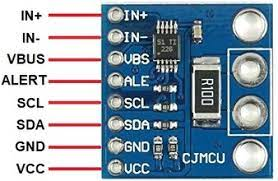
\includegraphics[width=5cm]{./img/INA226.jpeg}
	\caption{Capteur de tension et du courant INA226 }
	\label{i1}
\end{figure}

%%%\textbf{Caractéristiques principales :}
%\begin{filleditem}
%	\item Détecte les tensions de bus de 0 V à 26 V.
%	\item	Rapporte les tensions de shunt et de bus avec une haute précision.
%	\item	Précision de la tension de décalage : ± 80 µV (max).
%	\item	Erreur de gain : 0,25 % (max).
%	\item	Options de moyenne configurables.
%	\item	Quatre adresses programmables.
%	\item	Sorties d'alerte et d'avertissement programmables.
%	\item	Fonctionnement de l'alimentation : 2,7 V à 5,5 V.
%\\
%\end{filleditem}

\begin{filleditem}
	\item 	VCC : Il accepte une tension d'entrée de 2,7V à 5,5V,
	\item GND : Broche de terre, connectée à la masse de l'alimentation,
	\item SDA : Ligne de données série pour l'interface I2C. Elle est utilisée pour le transfert bidirectionnel de données,
	\item SCL : Ligne d'horloge série pour l'interface I2C. Elle est utilisée pour la synchronisation lors du transfert de données,
	\item ALE : il s'agit de la broche d'alerte,
	\item VBUS : Cette broche est utilisée pour mesurer la tension d'alimentation. Elle peut mesurer la tension d'alimentation jusqu'à 36 V,
	\item IN- : Cette broche se connecte à la charge. C'est là que la  résistance shunt est placée pour la détection du courant,
	\item IN+ : Cette broche se connecte à la source d'alimentation.\\
\end{filleditem}

%\subsection*{Avantages du INA3221}
%\begin{filleditem}
%	\item Multicanal : L'INA3221 peut surveiller simultanément la tension et le courant de trois sources distinctes, ce qui est idéal pour le projet où trois batteries solaires doivent être surveillées
	
%	\item	Efficacité : Utilisation d'un seul capteur pour plusieurs batteries réduit la complexité et le coût du système.
	
%	\item	Précision et fiabilité : Assure des mesures précises et fiables, cruciales pour la gestion optimale des batteries.
%\end{filleditem}

Le module est construit avec une puce INA226, quelques résistances et un condensateur qui aide à réduire le bruit ou les signaux électriques indésirables.

Voici le schéma du capteur :

\begin{figure}[H]
	\centering
	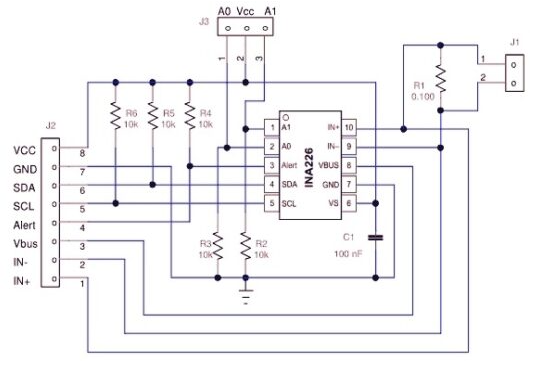
\includegraphics[width=12cm]{./img/schemabloc226.png}
	\caption{Schéma bloc de l'INA3221 }
	\label{i1}
\end{figure}


\subsection*{Système de traitement et d'envoi des données}
Le système de traitement constitue le cerveau central du système, où toutes les données capturées par les capteurs sont transmises pour être gérées, filtrées et analysées.\\
Cette phase de traitement assure plusieurs rôles cruciaux :
\begin{filleditem}
	\item \textbf{Gestion de la tension} : Contrôle des niveaux de tension pour maintenir la stabilité et éviter les surcharges ou les décharges excessives des batteries solaires.
	
	\item	\textbf{Gestion du courant} : Surveillance de courant pour optimiser l'efficacité énergétique et éviter les surcharges qui pourraient endommager les composants.
	
	\item	\textbf{Gestion de la température} : Contrôle des variations de température pour prévenir les effets néfastes sur les performances et la durée de vie des batteries.
	
	\item	\textbf{Gestion de la puissance} : Calcul et optimisation de la puissance générée et consommée par les batteries, en fonction des besoins énergétiques du système.
	
	\item	\textbf{Gestion de la charge et de la décharge} : Surveillance précise de l'état de charge (SoC) et de l'état de décharge (DoD) des batteries pour prolonger leur durée de vie et assurer une disponibilité continue.
	
	\item	\textbf{Gestion des alertes} : Détection et notification en temps réel des conditions anormales ou critiques, telles que les niveaux de tension et de température hors norme, pour permettre une intervention rapide et prévenir les défaillances potentielles.
	
	\item	\textbf{Envoi des données} : Transmission des données traitées et analysées vers une base de données en ligne ou un serveur distant, assurant ainsi une collecte centralisée et sécurisée des informations pour une surveillance continue et un suivi historique. 
\end{filleditem}

\subsection*{La carte électronique}
\subsection*{Arduino}
Arduino est une gamme de circuits électronique open source basée pour la plupart sur un micro-contrôleur du fabricant Atmel. Ces circuits intègrent les composants nécessaires pour permettre une utilisation rapide et simple du micro-contrôleur. cette simplification vise a rendre accessible à toute créations et programmation d'objet ou dispositifs interactifs . Il existe plusieurs types de carte Arduino mais pour notre cas , on va utiliser l'Arduino Mega car ce dernier comporte 16 pins analogique et 42 pins numériques. ces qui convient parfaitement au nombre des capteurs qu'on va utiliser lors de la réalisation.

\begin{figure}[H]
	\centering
	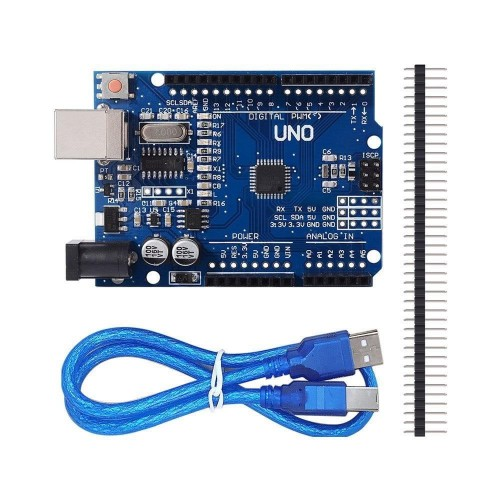
\includegraphics[width=8cm]{./img/arduinoAtmega.jpg}
	\caption{Module Arduino }
	\label{i1}
\end{figure}

\subsection*{Module GSM SIM808}

Le module est un téléphone GSM simple, sans clavier , écran , micro ni haut-parleur mais possédant une liaison série a connecter a un microcontrôleur local. Ce module prend en charge le réseau quadri bande GSM/GPRS et disponible pour la transmission et réception des SMS, de passer des appels. Ces qui fait la solution idéale de notre projet pour l'envoi des notification sous forme SMS aux utilisateur dans le cas anormaux.\\

\begin{figure}[H]
	\centering
	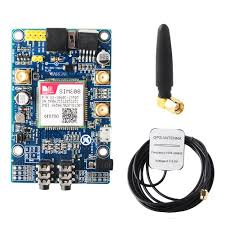
\includegraphics[width=6cm]{./img/gsmSim808.jpeg}
	\caption{Module GSM SIM808 }
	\label{i1}
\end{figure}

Caractéristique technique du SIM808: 
\begin{itemize}
	\item Alimentation 3,5 à 4,4 v,
	\item fréquence : 780MHz , 960MHz , 1710MHz , 2170MHz,
	\item effectuer et recevoir des appels vocaux à l'aide d'un casque et microphone externe,
	\item envoyer et recevoir des SMS,
	\item envoyer et de recevoir des données GPRS (TCP/IP , HTTP , etc),
	\item numériser et recevoir des émissions de radio FM,
	\item Dimensionnement 2.5cm x 2,3 cm x 0.7cm.
\end{itemize}


 
